\section{Performance of Annealing-based Quantum Computers}

\subsection{Hybrid DQM Solver}

This work sends the formulated DQM to a hybrid sampler at D-Wave for the optimizations using annealing-based hardware.
The hybrid sampler does not put the DQM on quantum hardware directly.
It classically searches the solution space.
The hybrid sampler speeds up this process by using quantum hardware to determine promising regions to explore next~\cite{DQMHybrid2020}.

The optimization of the DQM using the hybrid sampler for small problems seems to have linear time complexity.
If the UCP grows by $10$ time instances, the optimization takes about $0.1$ seconds longer.
Table \ref{table:evaluation.annealing.performance} lists the results of the optimizations and the time the hybrid sampler needed to achieve that result.
The optimization of these problems takes no longer than $5.6$ seconds each.

\begin{table}[ht]
  \centering
  \begin{tabular}{| r | r | r |}
  \hline 
  Number of Loads & Objective function & Time (in seconds) \\ 
  \hline \hline 
  10 & 487007.496 & 4.989 \\ \hline 
  20 & 817672.120 & 5.085 \\ \hline 
  25 & 681913.849 & 5.117 \\ \hline 
  30 & 1155685.053 & 5.215 \\ \hline 
  40 & 1554316.529 & 5.362 \\ \hline 
  50 & 1559508.051 & 5.510 \\ \hline 
\end{tabular}

  \caption{Results of Annealing Optimization with $4$ Power Plants}
  \label{table:evaluation.annealing.performance}
\end{table}

In figure \ref{figure:evaluation.annealing.performance} the time complexity is displayed clearer.
The time needed for optimizing problems with less than $15$ time instances also seems to be constant.
After that, the linear time complexity is visible.

When the problem size increases, the time complexity seems to be worse than linear.
This becomes clear in figure \ref{figure:evaluation.annealing.performance.extended}.
The time taken by the hybrid sampler to optimize the problem grows linearly but at a higher rate starting from $80$ time instances.
After this increase of slope, the slope stays the same until the problem size reaches $200$ time instances.
That is the maximum size of the UCP that this work considers on the hybrid DQM sampler.

\begin{figure}
  \begin{subfigure}[b]{0.5 \textwidth}
    \centering
    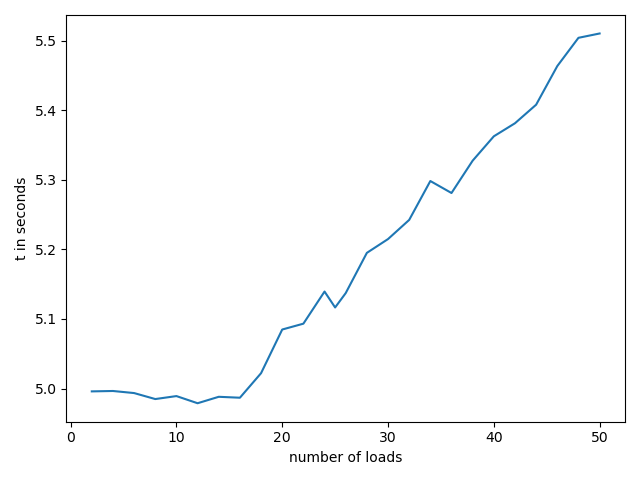
\includegraphics[width=\textwidth]{04_Validation/performance_annealing_p4.png}
    \caption{With up to $50$ Loads}
    \label{figure:evaluation.annealing.performance}
  \end{subfigure}
  \begin{subfigure}[b]{0.5 \textwidth}
    \centering
    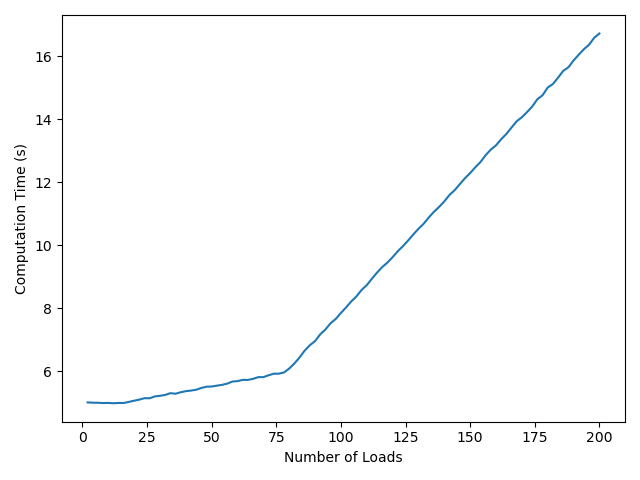
\includegraphics[width=\textwidth]{04_Validation/performance_annealing_p4_extended.png}
    \caption{With up to $200$ Loads}
    \label{figure:evaluation.annealing.performance.extended}
  \end{subfigure}
  \caption{Time Complexity of Annealing Optimization with $4$ Power Plants}
\end{figure}

The hybrid DQM sampler uses the minimum time specified by D-Wave for solving the problems.
D-Wave defines the minimum computing time for the hybrid DQM sampler with the pairs of density and time listed in table \ref{table:evaluation.dqm.hybrid.minimum.time}.
The sampler chooses the minimum computing time for a given DQM by interpolating linearly between the nearest two points.
Figure \ref{figure:evaluation.dqm.hybrid.minimum.time} shows the resulting function interpolating the points.
Figure \ref{figure:evaluation.dqm.hybrid.minimum.time.200} shows the part of the function corresponding to the experimental data in figure \ref{figure:evaluation.annealing.performance.extended} with the same unit --- number of time instances instead of density.
Figure \ref{figure:evaluation.annealing.performance.extended} and figure \ref{figure:evaluation.dqm.hybrid.minimum.time.200} are very similar.

\begin{table}[ht]
  \centering
  \begin{tabular}{| r | r |}
  \hline
  Density of DQM & Minimum Computing Time $t$ \\
  \hline \hline
  20000 & 5.0 \\
  \hline
  100000 & 6.0 \\
  \hline
  200000 & 13.0 \\
  \hline
  500000 & 34.0 \\
  \hline
  1000000 & 71.0 \\
  \hline
  2000000 & 152.0 \\
  \hline
  5000000 & 250.0 \\
  \hline
  20000000 & 400.0 \\
  \hline
  250000000 & 1200.0 \\
  \hline
\end{tabular}
  \caption{Interpolation Points for Minimum Computing Time of Hybrid DQM Solver}
  \label{table:evaluation.dqm.hybrid.minimum.time}
\end{table}

\begin{figure} [ht]
  \begin{subfigure}[b]{0.5 \textwidth}
    \centering
    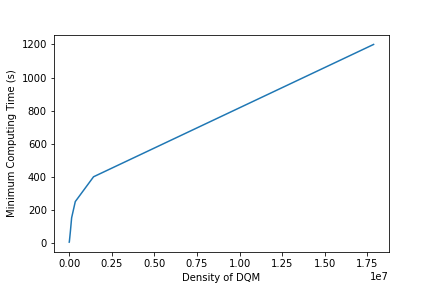
\includegraphics[width=\textwidth]{04_Validation/minimum_computing_time_dqm_hybrid.png}
    \caption{Full}
    \label{figure:evaluation.dqm.hybrid.minimum.time}
  \end{subfigure}
  \begin{subfigure}[b]{0.5 \textwidth}
    \centering
    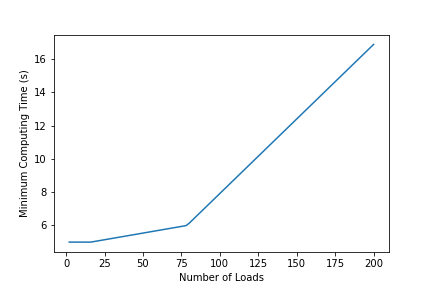
\includegraphics[width=\textwidth]{04_Validation/minimum_computing_time_dqm_hybrid_200.png}
    \caption{Corresponding to Extended Experiment Data}
    \label{figure:evaluation.dqm.hybrid.minimum.time.200}
  \end{subfigure}
  \caption{Minimum Computing Time of Hybrid DQM Solver}
\end{figure}

This approach does not produce optimal solutions for the UCP.
The summed power output of the single power plants does not meet the power demand because the DQM underestimates the demand part of the UCP.
After retrieving the optimal DQM solution and translating it to a UCP solution, the program adjusts the power outputs of the power plants.
It does so as described in section \ref{implementation:quantum.read.solution}.
That leads to a non-optimal solution of the UCP.

\subsubsection{Hybrid QUBO Solver}

This work implements the QUBOs for the UCP using the UQO-client.
Unfortunately, the access to D-Waves hybrid samplers are limited and this study used all the available computing time for the hybrid DQM sampler.
For this reason, this work does not consider the performance of the hybrid sampler for QUBOs.

Even though this work does not run the experiments on the hybrid QUBO sampler, the minimum computing power can be computed.
The hybrid QUBO sampler has a minimum computing time, just like the hybrid DQM sampler.
In this case, the computing time depends on the number of variables of the QUBO.
Table \ref{table:evaluation.qubo.hybrid.minimum.time} lists the pairs of variable amount and computing time.
Figure \ref{figure:evaluation.qubo.hybrid.minimum.time} shows the minimum time for all possible input sizes.
Figure \ref{figure:evaluation.qubo.hybrid.minimum.time.200} shows the minimum time for the experiments represented in figure \ref{figure:evaluation.annealing.performance.extended}.

\begin{table}[ht]
  \centering
  \begin{tabular}{| r | r |}
  \hline
  Number of Variables $v_{\text{QUBO}}$ & Minimum Computing Time $t$ (s) \\
  \hline \hline
  1 & 3.0 \\
  \hline
  1024 & 3.0 \\
  \hline
  4096 & 10.0 \\
  \hline
  10000 & 40.0 \\
  \hline
  30000 & 200.0 \\
  \hline
  100000 & 600.0 \\
  \hline
  1000000 & 600.0 \\
  \hline
  \end{tabular}
  \caption{Interpolation Points for Minimum Computing Time of Hybrid DQM Solver}
  \label{table:evaluation.qubo.hybrid.minimum.time}
\end{table}
\begin{figure} [ht]
  \begin{subfigure}[b]{0.5 \textwidth}
    \centering
    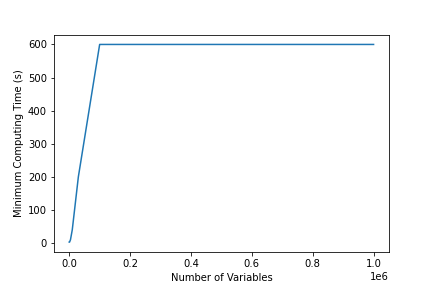
\includegraphics[width=\textwidth]{04_Validation/minimum_computing_time_qubo_hybrid.png}
    \caption{Full}
    \label{figure:evaluation.qubo.hybrid.minimum.time}
  \end{subfigure}
  \begin{subfigure}[b]{0.5 \textwidth}
    \centering
    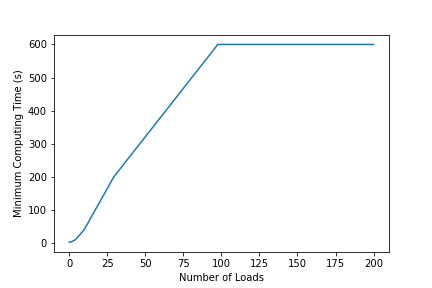
\includegraphics[width=\textwidth]{04_Validation/minimum_computing_time_qubo_hybrid_200.png}
    \caption{Corresponding to Extended Experiment Data}
    \label{figure:evaluation.qubo.hybrid.minimum.time.200}
  \end{subfigure}
  \caption{Minimum Computing Time of Hybrid QUBO Solver}
\end{figure}

The minimum computing time of this sampler is greater than the computing time of the hybrid DQM sampler for large inputs.
How much computing time this sampler would need additionally to the minimum computing time can't be reasoned about without actually performing experiments.

\subsubsection{Direct QUBO Solver}

D-Wave's QPUs can embed many QUBOs on them.
But if a QUBO has too many variables or quadratic biases connecting the biases, D-Wave might not find an embedding.
That is the case for the problems this work considers.

The smallest problem formulated as a QUBO has $1, 024$ variables and $263, 680$ quadratic biases.
These values can be calculated using formulas (\ref{formula:qubo.num.variables}) and (\ref{formula:qubo.num.quadratic.biases}) respectively.
One variable can have more than $255$ quadratic biases, also called a clique.
The reason is that power plant $4$ has $2^8$ possible power levels after discretizing the power levels, and variables for the different power levels of one power plant at one time instances are connected with quadratic biases.

Since the ``Advantage'' QPU has a $15$-way qubit connectivity, it would need an enormous amount of physical qubits to represent one logical binary variable.
More as there are available on the ``Advantage'' QPU~\cite{D-Wave2020, Zbinden2020}.
Because of this, the minor miner can't find embeddings for the QUBOs this work considers.
An algorithm designed specifically for embedding large cliques by \citeauthor{Zbinden2020} can not embed cliques larger than $180$ for the ''Pegasus'' architecture.
That implies that it is generally very hard or even impossible to find embeddings for QUBOs with cliques larger than $255$.
